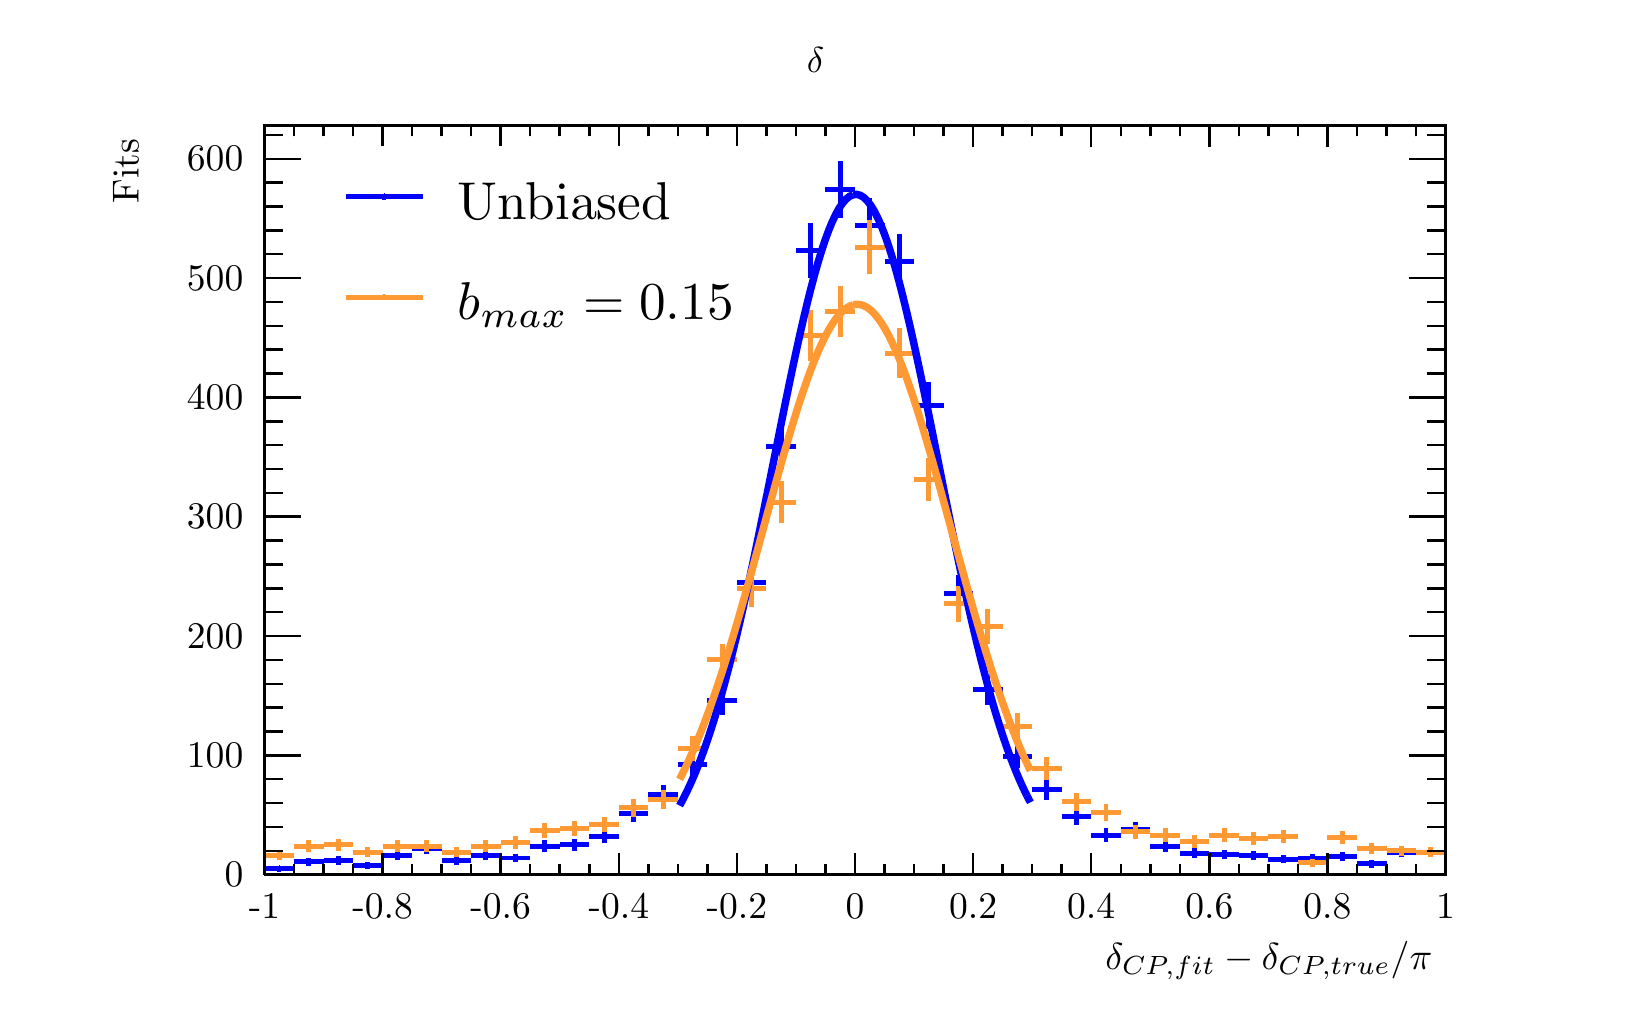
\begin{tikzpicture}
\pgfdeclareplotmark{cross} {
\pgfpathmoveto{\pgfpoint{-0.3\pgfplotmarksize}{\pgfplotmarksize}}
\pgfpathlineto{\pgfpoint{+0.3\pgfplotmarksize}{\pgfplotmarksize}}
\pgfpathlineto{\pgfpoint{+0.3\pgfplotmarksize}{0.3\pgfplotmarksize}}
\pgfpathlineto{\pgfpoint{+1\pgfplotmarksize}{0.3\pgfplotmarksize}}
\pgfpathlineto{\pgfpoint{+1\pgfplotmarksize}{-0.3\pgfplotmarksize}}
\pgfpathlineto{\pgfpoint{+0.3\pgfplotmarksize}{-0.3\pgfplotmarksize}}
\pgfpathlineto{\pgfpoint{+0.3\pgfplotmarksize}{-1.\pgfplotmarksize}}
\pgfpathlineto{\pgfpoint{-0.3\pgfplotmarksize}{-1.\pgfplotmarksize}}
\pgfpathlineto{\pgfpoint{-0.3\pgfplotmarksize}{-0.3\pgfplotmarksize}}
\pgfpathlineto{\pgfpoint{-1.\pgfplotmarksize}{-0.3\pgfplotmarksize}}
\pgfpathlineto{\pgfpoint{-1.\pgfplotmarksize}{0.3\pgfplotmarksize}}
\pgfpathlineto{\pgfpoint{-0.3\pgfplotmarksize}{0.3\pgfplotmarksize}}
\pgfpathclose
\pgfusepathqstroke
}
\pgfdeclareplotmark{cross*} {
\pgfpathmoveto{\pgfpoint{-0.3\pgfplotmarksize}{\pgfplotmarksize}}
\pgfpathlineto{\pgfpoint{+0.3\pgfplotmarksize}{\pgfplotmarksize}}
\pgfpathlineto{\pgfpoint{+0.3\pgfplotmarksize}{0.3\pgfplotmarksize}}
\pgfpathlineto{\pgfpoint{+1\pgfplotmarksize}{0.3\pgfplotmarksize}}
\pgfpathlineto{\pgfpoint{+1\pgfplotmarksize}{-0.3\pgfplotmarksize}}
\pgfpathlineto{\pgfpoint{+0.3\pgfplotmarksize}{-0.3\pgfplotmarksize}}
\pgfpathlineto{\pgfpoint{+0.3\pgfplotmarksize}{-1.\pgfplotmarksize}}
\pgfpathlineto{\pgfpoint{-0.3\pgfplotmarksize}{-1.\pgfplotmarksize}}
\pgfpathlineto{\pgfpoint{-0.3\pgfplotmarksize}{-0.3\pgfplotmarksize}}
\pgfpathlineto{\pgfpoint{-1.\pgfplotmarksize}{-0.3\pgfplotmarksize}}
\pgfpathlineto{\pgfpoint{-1.\pgfplotmarksize}{0.3\pgfplotmarksize}}
\pgfpathlineto{\pgfpoint{-0.3\pgfplotmarksize}{0.3\pgfplotmarksize}}
\pgfpathclose
\pgfusepathqfillstroke
}
\pgfdeclareplotmark{newstar} {
\pgfpathmoveto{\pgfqpoint{0pt}{\pgfplotmarksize}}
\pgfpathlineto{\pgfqpointpolar{44}{0.5\pgfplotmarksize}}
\pgfpathlineto{\pgfqpointpolar{18}{\pgfplotmarksize}}
\pgfpathlineto{\pgfqpointpolar{-20}{0.5\pgfplotmarksize}}
\pgfpathlineto{\pgfqpointpolar{-54}{\pgfplotmarksize}}
\pgfpathlineto{\pgfqpointpolar{-90}{0.5\pgfplotmarksize}}
\pgfpathlineto{\pgfqpointpolar{234}{\pgfplotmarksize}}
\pgfpathlineto{\pgfqpointpolar{198}{0.5\pgfplotmarksize}}
\pgfpathlineto{\pgfqpointpolar{162}{\pgfplotmarksize}}
\pgfpathlineto{\pgfqpointpolar{134}{0.5\pgfplotmarksize}}
\pgfpathclose
\pgfusepathqstroke
}
\pgfdeclareplotmark{newstar*} {
\pgfpathmoveto{\pgfqpoint{0pt}{\pgfplotmarksize}}
\pgfpathlineto{\pgfqpointpolar{44}{0.5\pgfplotmarksize}}
\pgfpathlineto{\pgfqpointpolar{18}{\pgfplotmarksize}}
\pgfpathlineto{\pgfqpointpolar{-20}{0.5\pgfplotmarksize}}
\pgfpathlineto{\pgfqpointpolar{-54}{\pgfplotmarksize}}
\pgfpathlineto{\pgfqpointpolar{-90}{0.5\pgfplotmarksize}}
\pgfpathlineto{\pgfqpointpolar{234}{\pgfplotmarksize}}
\pgfpathlineto{\pgfqpointpolar{198}{0.5\pgfplotmarksize}}
\pgfpathlineto{\pgfqpointpolar{162}{\pgfplotmarksize}}
\pgfpathlineto{\pgfqpointpolar{134}{0.5\pgfplotmarksize}}
\pgfpathclose
\pgfusepathqfillstroke
}
\definecolor{c}{rgb}{1,1,1};
\draw [color=c, fill=c] (0,0) rectangle (20,12.3567);
\draw [color=c, fill=c] (3,1.60637) rectangle (18,11.121);
\definecolor{c}{rgb}{0,0,0};
\draw [c,line width=0.9] (3,1.60637) -- (3,11.121) -- (18,11.121) -- (18,1.60637) -- (3,1.60637);
\definecolor{c}{rgb}{1,1,1};
\draw [color=c, fill=c] (3,1.60637) rectangle (18,11.121);
\definecolor{c}{rgb}{0,0,0};
\draw [c,line width=0.9] (3,1.60637) -- (3,11.121) -- (18,11.121) -- (18,1.60637) -- (3,1.60637);
\draw [c,line width=0.9] (3,1.60637) -- (18,1.60637);
\draw [c,line width=0.9] (3,1.88439) -- (3,1.60637);
\draw [c,line width=0.9] (3.375,1.74538) -- (3.375,1.60637);
\draw [c,line width=0.9] (3.75,1.74538) -- (3.75,1.60637);
\draw [c,line width=0.9] (4.125,1.74538) -- (4.125,1.60637);
\draw [c,line width=0.9] (4.5,1.88439) -- (4.5,1.60637);
\draw [c,line width=0.9] (4.875,1.74538) -- (4.875,1.60637);
\draw [c,line width=0.9] (5.25,1.74538) -- (5.25,1.60637);
\draw [c,line width=0.9] (5.625,1.74538) -- (5.625,1.60637);
\draw [c,line width=0.9] (6,1.88439) -- (6,1.60637);
\draw [c,line width=0.9] (6.375,1.74538) -- (6.375,1.60637);
\draw [c,line width=0.9] (6.75,1.74538) -- (6.75,1.60637);
\draw [c,line width=0.9] (7.125,1.74538) -- (7.125,1.60637);
\draw [c,line width=0.9] (7.5,1.88439) -- (7.5,1.60637);
\draw [c,line width=0.9] (7.875,1.74538) -- (7.875,1.60637);
\draw [c,line width=0.9] (8.25,1.74538) -- (8.25,1.60637);
\draw [c,line width=0.9] (8.625,1.74538) -- (8.625,1.60637);
\draw [c,line width=0.9] (9,1.88439) -- (9,1.60637);
\draw [c,line width=0.9] (9.375,1.74538) -- (9.375,1.60637);
\draw [c,line width=0.9] (9.75,1.74538) -- (9.75,1.60637);
\draw [c,line width=0.9] (10.125,1.74538) -- (10.125,1.60637);
\draw [c,line width=0.9] (10.5,1.88439) -- (10.5,1.60637);
\draw [c,line width=0.9] (10.875,1.74538) -- (10.875,1.60637);
\draw [c,line width=0.9] (11.25,1.74538) -- (11.25,1.60637);
\draw [c,line width=0.9] (11.625,1.74538) -- (11.625,1.60637);
\draw [c,line width=0.9] (12,1.88439) -- (12,1.60637);
\draw [c,line width=0.9] (12.375,1.74538) -- (12.375,1.60637);
\draw [c,line width=0.9] (12.75,1.74538) -- (12.75,1.60637);
\draw [c,line width=0.9] (13.125,1.74538) -- (13.125,1.60637);
\draw [c,line width=0.9] (13.5,1.88439) -- (13.5,1.60637);
\draw [c,line width=0.9] (13.875,1.74538) -- (13.875,1.60637);
\draw [c,line width=0.9] (14.25,1.74538) -- (14.25,1.60637);
\draw [c,line width=0.9] (14.625,1.74538) -- (14.625,1.60637);
\draw [c,line width=0.9] (15,1.88439) -- (15,1.60637);
\draw [c,line width=0.9] (15.375,1.74538) -- (15.375,1.60637);
\draw [c,line width=0.9] (15.75,1.74538) -- (15.75,1.60637);
\draw [c,line width=0.9] (16.125,1.74538) -- (16.125,1.60637);
\draw [c,line width=0.9] (16.5,1.88439) -- (16.5,1.60637);
\draw [c,line width=0.9] (16.875,1.74538) -- (16.875,1.60637);
\draw [c,line width=0.9] (17.25,1.74538) -- (17.25,1.60637);
\draw [c,line width=0.9] (17.625,1.74538) -- (17.625,1.60637);
\draw [c,line width=0.9] (18,1.88439) -- (18,1.60637);
\draw [c,line width=0.9] (3,1.88439) -- (3,1.60637);
\draw [c,line width=0.9] (18,1.88439) -- (18,1.60637);
\draw [anchor=base] (3,1.05032) node[scale=1.35805, color=c, rotate=0]{-1};
\draw [anchor=base] (4.5,1.05032) node[scale=1.35805, color=c, rotate=0]{-0.8};
\draw [anchor=base] (6,1.05032) node[scale=1.35805, color=c, rotate=0]{-0.6};
\draw [anchor=base] (7.5,1.05032) node[scale=1.35805, color=c, rotate=0]{-0.4};
\draw [anchor=base] (9,1.05032) node[scale=1.35805, color=c, rotate=0]{-0.2};
\draw [anchor=base] (10.5,1.05032) node[scale=1.35805, color=c, rotate=0]{0};
\draw [anchor=base] (12,1.05032) node[scale=1.35805, color=c, rotate=0]{0.2};
\draw [anchor=base] (13.5,1.05032) node[scale=1.35805, color=c, rotate=0]{0.4};
\draw [anchor=base] (15,1.05032) node[scale=1.35805, color=c, rotate=0]{0.6};
\draw [anchor=base] (16.5,1.05032) node[scale=1.35805, color=c, rotate=0]{0.8};
\draw [anchor=base] (18,1.05032) node[scale=1.35805, color=c, rotate=0]{1};
\draw [anchor= east] (18,0.518981) node[scale=1.35805, color=c, rotate=0]{$ \delta_{CP, fit} - \delta_{CP, true} / \pi$};
\draw [c,line width=0.9] (3,11.121) -- (18,11.121);
\draw [c,line width=0.9] (3,10.843) -- (3,11.121);
\draw [c,line width=0.9] (3.375,10.982) -- (3.375,11.121);
\draw [c,line width=0.9] (3.75,10.982) -- (3.75,11.121);
\draw [c,line width=0.9] (4.125,10.982) -- (4.125,11.121);
\draw [c,line width=0.9] (4.5,10.843) -- (4.5,11.121);
\draw [c,line width=0.9] (4.875,10.982) -- (4.875,11.121);
\draw [c,line width=0.9] (5.25,10.982) -- (5.25,11.121);
\draw [c,line width=0.9] (5.625,10.982) -- (5.625,11.121);
\draw [c,line width=0.9] (6,10.843) -- (6,11.121);
\draw [c,line width=0.9] (6.375,10.982) -- (6.375,11.121);
\draw [c,line width=0.9] (6.75,10.982) -- (6.75,11.121);
\draw [c,line width=0.9] (7.125,10.982) -- (7.125,11.121);
\draw [c,line width=0.9] (7.5,10.843) -- (7.5,11.121);
\draw [c,line width=0.9] (7.875,10.982) -- (7.875,11.121);
\draw [c,line width=0.9] (8.25,10.982) -- (8.25,11.121);
\draw [c,line width=0.9] (8.625,10.982) -- (8.625,11.121);
\draw [c,line width=0.9] (9,10.843) -- (9,11.121);
\draw [c,line width=0.9] (9.375,10.982) -- (9.375,11.121);
\draw [c,line width=0.9] (9.75,10.982) -- (9.75,11.121);
\draw [c,line width=0.9] (10.125,10.982) -- (10.125,11.121);
\draw [c,line width=0.9] (10.5,10.843) -- (10.5,11.121);
\draw [c,line width=0.9] (10.875,10.982) -- (10.875,11.121);
\draw [c,line width=0.9] (11.25,10.982) -- (11.25,11.121);
\draw [c,line width=0.9] (11.625,10.982) -- (11.625,11.121);
\draw [c,line width=0.9] (12,10.843) -- (12,11.121);
\draw [c,line width=0.9] (12.375,10.982) -- (12.375,11.121);
\draw [c,line width=0.9] (12.75,10.982) -- (12.75,11.121);
\draw [c,line width=0.9] (13.125,10.982) -- (13.125,11.121);
\draw [c,line width=0.9] (13.5,10.843) -- (13.5,11.121);
\draw [c,line width=0.9] (13.875,10.982) -- (13.875,11.121);
\draw [c,line width=0.9] (14.25,10.982) -- (14.25,11.121);
\draw [c,line width=0.9] (14.625,10.982) -- (14.625,11.121);
\draw [c,line width=0.9] (15,10.843) -- (15,11.121);
\draw [c,line width=0.9] (15.375,10.982) -- (15.375,11.121);
\draw [c,line width=0.9] (15.75,10.982) -- (15.75,11.121);
\draw [c,line width=0.9] (16.125,10.982) -- (16.125,11.121);
\draw [c,line width=0.9] (16.5,10.843) -- (16.5,11.121);
\draw [c,line width=0.9] (16.875,10.982) -- (16.875,11.121);
\draw [c,line width=0.9] (17.25,10.982) -- (17.25,11.121);
\draw [c,line width=0.9] (17.625,10.982) -- (17.625,11.121);
\draw [c,line width=0.9] (18,10.843) -- (18,11.121);
\draw [c,line width=0.9] (3,10.843) -- (3,11.121);
\draw [c,line width=0.9] (18,10.843) -- (18,11.121);
\draw [c,line width=0.9] (3,1.60637) -- (3,11.121);
\draw [c,line width=0.9] (3.462,1.60637) -- (3,1.60637);
\draw [c,line width=0.9] (3.231,1.90945) -- (3,1.90945);
\draw [c,line width=0.9] (3.231,2.21254) -- (3,2.21254);
\draw [c,line width=0.9] (3.231,2.51562) -- (3,2.51562);
\draw [c,line width=0.9] (3.231,2.8187) -- (3,2.8187);
\draw [c,line width=0.9] (3.462,3.12179) -- (3,3.12179);
\draw [c,line width=0.9] (3.231,3.42487) -- (3,3.42487);
\draw [c,line width=0.9] (3.231,3.72796) -- (3,3.72796);
\draw [c,line width=0.9] (3.231,4.03104) -- (3,4.03104);
\draw [c,line width=0.9] (3.231,4.33412) -- (3,4.33412);
\draw [c,line width=0.9] (3.462,4.63721) -- (3,4.63721);
\draw [c,line width=0.9] (3.231,4.94029) -- (3,4.94029);
\draw [c,line width=0.9] (3.231,5.24337) -- (3,5.24337);
\draw [c,line width=0.9] (3.231,5.54646) -- (3,5.54646);
\draw [c,line width=0.9] (3.231,5.84954) -- (3,5.84954);
\draw [c,line width=0.9] (3.462,6.15263) -- (3,6.15263);
\draw [c,line width=0.9] (3.231,6.45571) -- (3,6.45571);
\draw [c,line width=0.9] (3.231,6.75879) -- (3,6.75879);
\draw [c,line width=0.9] (3.231,7.06188) -- (3,7.06188);
\draw [c,line width=0.9] (3.231,7.36496) -- (3,7.36496);
\draw [c,line width=0.9] (3.462,7.66804) -- (3,7.66804);
\draw [c,line width=0.9] (3.231,7.97113) -- (3,7.97113);
\draw [c,line width=0.9] (3.231,8.27421) -- (3,8.27421);
\draw [c,line width=0.9] (3.231,8.57729) -- (3,8.57729);
\draw [c,line width=0.9] (3.231,8.88038) -- (3,8.88038);
\draw [c,line width=0.9] (3.462,9.18346) -- (3,9.18346);
\draw [c,line width=0.9] (3.231,9.48655) -- (3,9.48655);
\draw [c,line width=0.9] (3.231,9.78963) -- (3,9.78963);
\draw [c,line width=0.9] (3.231,10.0927) -- (3,10.0927);
\draw [c,line width=0.9] (3.231,10.3958) -- (3,10.3958);
\draw [c,line width=0.9] (3.462,10.6989) -- (3,10.6989);
\draw [c,line width=0.9] (3.462,10.6989) -- (3,10.6989);
\draw [c,line width=0.9] (3.231,11.002) -- (3,11.002);
\draw [anchor= east] (2.9,1.60637) node[scale=1.35805, color=c, rotate=0]{0};
\draw [anchor= east] (2.9,3.12179) node[scale=1.35805, color=c, rotate=0]{100};
\draw [anchor= east] (2.9,4.63721) node[scale=1.35805, color=c, rotate=0]{200};
\draw [anchor= east] (2.9,6.15263) node[scale=1.35805, color=c, rotate=0]{300};
\draw [anchor= east] (2.9,7.66804) node[scale=1.35805, color=c, rotate=0]{400};
\draw [anchor= east] (2.9,9.18346) node[scale=1.35805, color=c, rotate=0]{500};
\draw [anchor= east] (2.9,10.6989) node[scale=1.35805, color=c, rotate=0]{600};
\draw [anchor= east] (1.24,11.121) node[scale=1.35805, color=c, rotate=90]{ Fits};
\draw [c,line width=0.9] (18,1.60637) -- (18,11.121);
\draw [c,line width=0.9] (17.538,1.60637) -- (18,1.60637);
\draw [c,line width=0.9] (17.769,1.90945) -- (18,1.90945);
\draw [c,line width=0.9] (17.769,2.21254) -- (18,2.21254);
\draw [c,line width=0.9] (17.769,2.51562) -- (18,2.51562);
\draw [c,line width=0.9] (17.769,2.8187) -- (18,2.8187);
\draw [c,line width=0.9] (17.538,3.12179) -- (18,3.12179);
\draw [c,line width=0.9] (17.769,3.42487) -- (18,3.42487);
\draw [c,line width=0.9] (17.769,3.72796) -- (18,3.72796);
\draw [c,line width=0.9] (17.769,4.03104) -- (18,4.03104);
\draw [c,line width=0.9] (17.769,4.33412) -- (18,4.33412);
\draw [c,line width=0.9] (17.538,4.63721) -- (18,4.63721);
\draw [c,line width=0.9] (17.769,4.94029) -- (18,4.94029);
\draw [c,line width=0.9] (17.769,5.24337) -- (18,5.24337);
\draw [c,line width=0.9] (17.769,5.54646) -- (18,5.54646);
\draw [c,line width=0.9] (17.769,5.84954) -- (18,5.84954);
\draw [c,line width=0.9] (17.538,6.15263) -- (18,6.15263);
\draw [c,line width=0.9] (17.769,6.45571) -- (18,6.45571);
\draw [c,line width=0.9] (17.769,6.75879) -- (18,6.75879);
\draw [c,line width=0.9] (17.769,7.06188) -- (18,7.06188);
\draw [c,line width=0.9] (17.769,7.36496) -- (18,7.36496);
\draw [c,line width=0.9] (17.538,7.66804) -- (18,7.66804);
\draw [c,line width=0.9] (17.769,7.97113) -- (18,7.97113);
\draw [c,line width=0.9] (17.769,8.27421) -- (18,8.27421);
\draw [c,line width=0.9] (17.769,8.57729) -- (18,8.57729);
\draw [c,line width=0.9] (17.769,8.88038) -- (18,8.88038);
\draw [c,line width=0.9] (17.538,9.18346) -- (18,9.18346);
\draw [c,line width=0.9] (17.769,9.48655) -- (18,9.48655);
\draw [c,line width=0.9] (17.769,9.78963) -- (18,9.78963);
\draw [c,line width=0.9] (17.769,10.0927) -- (18,10.0927);
\draw [c,line width=0.9] (17.769,10.3958) -- (18,10.3958);
\draw [c,line width=0.9] (17.538,10.6989) -- (18,10.6989);
\draw [c,line width=0.9] (17.538,10.6989) -- (18,10.6989);
\draw [c,line width=0.9] (17.769,11.002) -- (18,11.002);
\definecolor{c}{rgb}{0,0,1};
\draw [c,line width=1.8] (3.1875,1.64825) -- (3.1875,1.68214);
\draw [c,line width=1.8] (3.1875,1.68214) -- (3.1875,1.71603);
\draw [c,line width=1.8] (3,1.68214) -- (3.1875,1.68214);
\draw [c,line width=1.8] (3.1875,1.68214) -- (3.375,1.68214);
\foreach \P in {(3.1875,1.68214)}{\draw[mark options={color=c,fill=c},mark size=2.402402pt, line width=0.000000pt, mark=*,mark size=1pt] plot coordinates {\P};}
\draw [c,line width=1.8] (3.5625,1.7228) -- (3.5625,1.77307);
\draw [c,line width=1.8] (3.5625,1.77307) -- (3.5625,1.82333);
\draw [c,line width=1.8] (3.375,1.77307) -- (3.5625,1.77307);
\draw [c,line width=1.8] (3.5625,1.77307) -- (3.75,1.77307);
\foreach \P in {(3.5625,1.77307)}{\draw[mark options={color=c,fill=c},mark size=2.402402pt, line width=0.000000pt, mark=*,mark size=1pt] plot coordinates {\P};}
\draw [c,line width=1.8] (3.9375,1.73572) -- (3.9375,1.78822);
\draw [c,line width=1.8] (3.9375,1.78822) -- (3.9375,1.84072);
\draw [c,line width=1.8] (3.75,1.78822) -- (3.9375,1.78822);
\draw [c,line width=1.8] (3.9375,1.78822) -- (4.125,1.78822);
\foreach \P in {(3.9375,1.78822)}{\draw[mark options={color=c,fill=c},mark size=2.402402pt, line width=0.000000pt, mark=*,mark size=1pt] plot coordinates {\P};}
\draw [c,line width=1.8] (4.3125,1.68474) -- (4.3125,1.7276);
\draw [c,line width=1.8] (4.3125,1.7276) -- (4.3125,1.77047);
\draw [c,line width=1.8] (4.125,1.7276) -- (4.3125,1.7276);
\draw [c,line width=1.8] (4.3125,1.7276) -- (4.5,1.7276);
\foreach \P in {(4.3125,1.7276)}{\draw[mark options={color=c,fill=c},mark size=2.402402pt, line width=0.000000pt, mark=*,mark size=1pt] plot coordinates {\P};}
\draw [c,line width=1.8] (4.6875,1.78822) -- (4.6875,1.84884);
\draw [c,line width=1.8] (4.6875,1.84884) -- (4.6875,1.90945);
\draw [c,line width=1.8] (4.5,1.84884) -- (4.6875,1.84884);
\draw [c,line width=1.8] (4.6875,1.84884) -- (4.875,1.84884);
\foreach \P in {(4.6875,1.84884)}{\draw[mark options={color=c,fill=c},mark size=2.402402pt, line width=0.000000pt, mark=*,mark size=1pt] plot coordinates {\P};}
\draw [c,line width=1.8] (5.0625,1.86868) -- (5.0625,1.93976);
\draw [c,line width=1.8] (5.0625,1.93976) -- (5.0625,2.01084);
\draw [c,line width=1.8] (4.875,1.93976) -- (5.0625,1.93976);
\draw [c,line width=1.8] (5.0625,1.93976) -- (5.25,1.93976);
\foreach \P in {(5.0625,1.93976)}{\draw[mark options={color=c,fill=c},mark size=2.402402pt, line width=0.000000pt, mark=*,mark size=1pt] plot coordinates {\P};}
\draw [c,line width=1.8] (5.4375,1.73572) -- (5.4375,1.78822);
\draw [c,line width=1.8] (5.4375,1.78822) -- (5.4375,1.84072);
\draw [c,line width=1.8] (5.25,1.78822) -- (5.4375,1.78822);
\draw [c,line width=1.8] (5.4375,1.78822) -- (5.625,1.78822);
\foreach \P in {(5.4375,1.78822)}{\draw[mark options={color=c,fill=c},mark size=2.402402pt, line width=0.000000pt, mark=*,mark size=1pt] plot coordinates {\P};}
\draw [c,line width=1.8] (5.8125,1.78822) -- (5.8125,1.84884);
\draw [c,line width=1.8] (5.8125,1.84884) -- (5.8125,1.90945);
\draw [c,line width=1.8] (5.625,1.84884) -- (5.8125,1.84884);
\draw [c,line width=1.8] (5.8125,1.84884) -- (6,1.84884);
\foreach \P in {(5.8125,1.84884)}{\draw[mark options={color=c,fill=c},mark size=2.402402pt, line width=0.000000pt, mark=*,mark size=1pt] plot coordinates {\P};}
\draw [c,line width=1.8] (6.1875,1.76183) -- (6.1875,1.81853);
\draw [c,line width=1.8] (6.1875,1.81853) -- (6.1875,1.87523);
\draw [c,line width=1.8] (6,1.81853) -- (6.1875,1.81853);
\draw [c,line width=1.8] (6.1875,1.81853) -- (6.375,1.81853);
\foreach \P in {(6.1875,1.81853)}{\draw[mark options={color=c,fill=c},mark size=2.402402pt, line width=0.000000pt, mark=*,mark size=1pt] plot coordinates {\P};}
\draw [c,line width=1.8] (6.5625,1.89583) -- (6.5625,1.97007);
\draw [c,line width=1.8] (6.5625,1.97007) -- (6.5625,2.04431);
\draw [c,line width=1.8] (6.375,1.97007) -- (6.5625,1.97007);
\draw [c,line width=1.8] (6.5625,1.97007) -- (6.75,1.97007);
\foreach \P in {(6.5625,1.97007)}{\draw[mark options={color=c,fill=c},mark size=2.402402pt, line width=0.000000pt, mark=*,mark size=1pt] plot coordinates {\P};}
\draw [c,line width=1.8] (6.9375,1.90945) -- (6.9375,1.98522);
\draw [c,line width=1.8] (6.9375,1.98522) -- (6.9375,2.06099);
\draw [c,line width=1.8] (6.75,1.98522) -- (6.9375,1.98522);
\draw [c,line width=1.8] (6.9375,1.98522) -- (7.125,1.98522);
\foreach \P in {(6.9375,1.98522)}{\draw[mark options={color=c,fill=c},mark size=2.402402pt, line width=0.000000pt, mark=*,mark size=1pt] plot coordinates {\P};}
\draw [c,line width=1.8] (7.3125,2.00558) -- (7.3125,2.0913);
\draw [c,line width=1.8] (7.3125,2.0913) -- (7.3125,2.17703);
\draw [c,line width=1.8] (7.125,2.0913) -- (7.3125,2.0913);
\draw [c,line width=1.8] (7.3125,2.0913) -- (7.5,2.0913);
\foreach \P in {(7.3125,2.0913)}{\draw[mark options={color=c,fill=c},mark size=2.402402pt, line width=0.000000pt, mark=*,mark size=1pt] plot coordinates {\P};}
\draw [c,line width=1.8] (7.6875,2.27101) -- (7.6875,2.37923);
\draw [c,line width=1.8] (7.6875,2.37923) -- (7.6875,2.48746);
\draw [c,line width=1.8] (7.5,2.37923) -- (7.6875,2.37923);
\draw [c,line width=1.8] (7.6875,2.37923) -- (7.875,2.37923);
\foreach \P in {(7.6875,2.37923)}{\draw[mark options={color=c,fill=c},mark size=2.402402pt, line width=0.000000pt, mark=*,mark size=1pt] plot coordinates {\P};}
\draw [c,line width=1.8] (8.0625,2.49766) -- (8.0625,2.6217);
\draw [c,line width=1.8] (8.0625,2.6217) -- (8.0625,2.74574);
\draw [c,line width=1.8] (7.875,2.6217) -- (8.0625,2.6217);
\draw [c,line width=1.8] (8.0625,2.6217) -- (8.25,2.6217);
\foreach \P in {(8.0625,2.6217)}{\draw[mark options={color=c,fill=c},mark size=2.402402pt, line width=0.000000pt, mark=*,mark size=1pt] plot coordinates {\P};}
\draw [c,line width=1.8] (8.4375,2.8552) -- (8.4375,3.00055);
\draw [c,line width=1.8] (8.4375,3.00055) -- (8.4375,3.14591);
\draw [c,line width=1.8] (8.25,3.00055) -- (8.4375,3.00055);
\draw [c,line width=1.8] (8.4375,3.00055) -- (8.625,3.00055);
\foreach \P in {(8.4375,3.00055)}{\draw[mark options={color=c,fill=c},mark size=2.402402pt, line width=0.000000pt, mark=*,mark size=1pt] plot coordinates {\P};}
\draw [c,line width=1.8] (8.8125,3.63577) -- (8.8125,3.81888);
\draw [c,line width=1.8] (8.8125,3.81888) -- (8.8125,4.00199);
\draw [c,line width=1.8] (8.625,3.81888) -- (8.8125,3.81888);
\draw [c,line width=1.8] (8.8125,3.81888) -- (9,3.81888);
\foreach \P in {(8.8125,3.81888)}{\draw[mark options={color=c,fill=c},mark size=2.402402pt, line width=0.000000pt, mark=*,mark size=1pt] plot coordinates {\P};}
\draw [c,line width=1.8] (9.1875,5.08194) -- (9.1875,5.31914);
\draw [c,line width=1.8] (9.1875,5.31914) -- (9.1875,5.55635);
\draw [c,line width=1.8] (9,5.31914) -- (9.1875,5.31914);
\draw [c,line width=1.8] (9.1875,5.31914) -- (9.375,5.31914);
\foreach \P in {(9.1875,5.31914)}{\draw[mark options={color=c,fill=c},mark size=2.402402pt, line width=0.000000pt, mark=*,mark size=1pt] plot coordinates {\P};}
\draw [c,line width=1.8] (9.5625,6.75959) -- (9.5625,7.04672);
\draw [c,line width=1.8] (9.5625,7.04672) -- (9.5625,7.33385);
\draw [c,line width=1.8] (9.375,7.04672) -- (9.5625,7.04672);
\draw [c,line width=1.8] (9.5625,7.04672) -- (9.75,7.04672);
\foreach \P in {(9.5625,7.04672)}{\draw[mark options={color=c,fill=c},mark size=2.402402pt, line width=0.000000pt, mark=*,mark size=1pt] plot coordinates {\P};}
\draw [c,line width=1.8] (9.9375,9.18544) -- (9.9375,9.53201);
\draw [c,line width=1.8] (9.9375,9.53201) -- (9.9375,9.87857);
\draw [c,line width=1.8] (9.75,9.53201) -- (9.9375,9.53201);
\draw [c,line width=1.8] (9.9375,9.53201) -- (10.125,9.53201);
\foreach \P in {(9.9375,9.53201)}{\draw[mark options={color=c,fill=c},mark size=2.402402pt, line width=0.000000pt, mark=*,mark size=1pt] plot coordinates {\P};}
\draw [c,line width=1.8] (10.3125,9.9418) -- (10.3125,10.3049);
\draw [c,line width=1.8] (10.3125,10.3049) -- (10.3125,10.6679);
\draw [c,line width=1.8] (10.125,10.3049) -- (10.3125,10.3049);
\draw [c,line width=1.8] (10.3125,10.3049) -- (10.5,10.3049);
\foreach \P in {(10.3125,10.3049)}{\draw[mark options={color=c,fill=c},mark size=2.402402pt, line width=0.000000pt, mark=*,mark size=1pt] plot coordinates {\P};}
\draw [c,line width=1.8] (10.6875,9.49679) -- (10.6875,9.85025);
\draw [c,line width=1.8] (10.6875,9.85025) -- (10.6875,10.2037);
\draw [c,line width=1.8] (10.5,9.85025) -- (10.6875,9.85025);
\draw [c,line width=1.8] (10.6875,9.85025) -- (10.875,9.85025);
\foreach \P in {(10.6875,9.85025)}{\draw[mark options={color=c,fill=c},mark size=2.402402pt, line width=0.000000pt, mark=*,mark size=1pt] plot coordinates {\P};}
\draw [c,line width=1.8] (11.0625,9.05205) -- (11.0625,9.39562);
\draw [c,line width=1.8] (11.0625,9.39562) -- (11.0625,9.73919);
\draw [c,line width=1.8] (10.875,9.39562) -- (11.0625,9.39562);
\draw [c,line width=1.8] (11.0625,9.39562) -- (11.25,9.39562);
\foreach \P in {(11.0625,9.39562)}{\draw[mark options={color=c,fill=c},mark size=2.402402pt, line width=0.000000pt, mark=*,mark size=1pt] plot coordinates {\P};}
\draw [c,line width=1.8] (11.4375,7.26154) -- (11.4375,7.56196);
\draw [c,line width=1.8] (11.4375,7.56196) -- (11.4375,7.86238);
\draw [c,line width=1.8] (11.25,7.56196) -- (11.4375,7.56196);
\draw [c,line width=1.8] (11.4375,7.56196) -- (11.625,7.56196);
\foreach \P in {(11.4375,7.56196)}{\draw[mark options={color=c,fill=c},mark size=2.402402pt, line width=0.000000pt, mark=*,mark size=1pt] plot coordinates {\P};}
\draw [c,line width=1.8] (11.8125,4.94995) -- (11.8125,5.18276);
\draw [c,line width=1.8] (11.8125,5.18276) -- (11.8125,5.41556);
\draw [c,line width=1.8] (11.625,5.18276) -- (11.8125,5.18276);
\draw [c,line width=1.8] (11.8125,5.18276) -- (12,5.18276);
\foreach \P in {(11.8125,5.18276)}{\draw[mark options={color=c,fill=c},mark size=2.402402pt, line width=0.000000pt, mark=*,mark size=1pt] plot coordinates {\P};}
\draw [c,line width=1.8] (12.1875,3.7666) -- (12.1875,3.95527);
\draw [c,line width=1.8] (12.1875,3.95527) -- (12.1875,4.14394);
\draw [c,line width=1.8] (12,3.95527) -- (12.1875,3.95527);
\draw [c,line width=1.8] (12.1875,3.95527) -- (12.375,3.95527);
\foreach \P in {(12.1875,3.95527)}{\draw[mark options={color=c,fill=c},mark size=2.402402pt, line width=0.000000pt, mark=*,mark size=1pt] plot coordinates {\P};}
\draw [c,line width=1.8] (12.5625,2.95585) -- (12.5625,3.10663);
\draw [c,line width=1.8] (12.5625,3.10663) -- (12.5625,3.25742);
\draw [c,line width=1.8] (12.375,3.10663) -- (12.5625,3.10663);
\draw [c,line width=1.8] (12.5625,3.10663) -- (12.75,3.10663);
\foreach \P in {(12.5625,3.10663)}{\draw[mark options={color=c,fill=c},mark size=2.402402pt, line width=0.000000pt, mark=*,mark size=1pt] plot coordinates {\P};}
\draw [c,line width=1.8] (12.9375,2.55463) -- (12.9375,2.68232);
\draw [c,line width=1.8] (12.9375,2.68232) -- (12.9375,2.81001);
\draw [c,line width=1.8] (12.75,2.68232) -- (12.9375,2.68232);
\draw [c,line width=1.8] (12.9375,2.68232) -- (13.125,2.68232);
\foreach \P in {(12.9375,2.68232)}{\draw[mark options={color=c,fill=c},mark size=2.402402pt, line width=0.000000pt, mark=*,mark size=1pt] plot coordinates {\P};}
\draw [c,line width=1.8] (13.3125,2.24285) -- (13.3125,2.34892);
\draw [c,line width=1.8] (13.3125,2.34892) -- (13.3125,2.455);
\draw [c,line width=1.8] (13.125,2.34892) -- (13.3125,2.34892);
\draw [c,line width=1.8] (13.3125,2.34892) -- (13.5,2.34892);
\foreach \P in {(13.3125,2.34892)}{\draw[mark options={color=c,fill=c},mark size=2.402402pt, line width=0.000000pt, mark=*,mark size=1pt] plot coordinates {\P};}
\draw [c,line width=1.8] (13.6875,2.0194) -- (13.6875,2.10646);
\draw [c,line width=1.8] (13.6875,2.10646) -- (13.6875,2.19351);
\draw [c,line width=1.8] (13.5,2.10646) -- (13.6875,2.10646);
\draw [c,line width=1.8] (13.6875,2.10646) -- (13.875,2.10646);
\foreach \P in {(13.6875,2.10646)}{\draw[mark options={color=c,fill=c},mark size=2.402402pt, line width=0.000000pt, mark=*,mark size=1pt] plot coordinates {\P};}
\draw [c,line width=1.8] (14.0625,2.08881) -- (14.0625,2.18223);
\draw [c,line width=1.8] (14.0625,2.18223) -- (14.0625,2.27565);
\draw [c,line width=1.8] (13.875,2.18223) -- (14.0625,2.18223);
\draw [c,line width=1.8] (14.0625,2.18223) -- (14.25,2.18223);
\foreach \P in {(14.0625,2.18223)}{\draw[mark options={color=c,fill=c},mark size=2.402402pt, line width=0.000000pt, mark=*,mark size=1pt] plot coordinates {\P};}
\draw [c,line width=1.8] (14.4375,1.89583) -- (14.4375,1.97007);
\draw [c,line width=1.8] (14.4375,1.97007) -- (14.4375,2.04431);
\draw [c,line width=1.8] (14.25,1.97007) -- (14.4375,1.97007);
\draw [c,line width=1.8] (14.4375,1.97007) -- (14.625,1.97007);
\foreach \P in {(14.4375,1.97007)}{\draw[mark options={color=c,fill=c},mark size=2.402402pt, line width=0.000000pt, mark=*,mark size=1pt] plot coordinates {\P};}
\draw [c,line width=1.8] (14.8125,1.81485) -- (14.8125,1.87914);
\draw [c,line width=1.8] (14.8125,1.87914) -- (14.8125,1.94344);
\draw [c,line width=1.8] (14.625,1.87914) -- (14.8125,1.87914);
\draw [c,line width=1.8] (14.8125,1.87914) -- (15,1.87914);
\foreach \P in {(14.8125,1.87914)}{\draw[mark options={color=c,fill=c},mark size=2.402402pt, line width=0.000000pt, mark=*,mark size=1pt] plot coordinates {\P};}
\draw [c,line width=1.8] (15.1875,1.80151) -- (15.1875,1.86399);
\draw [c,line width=1.8] (15.1875,1.86399) -- (15.1875,1.92647);
\draw [c,line width=1.8] (15,1.86399) -- (15.1875,1.86399);
\draw [c,line width=1.8] (15.1875,1.86399) -- (15.375,1.86399);
\foreach \P in {(15.1875,1.86399)}{\draw[mark options={color=c,fill=c},mark size=2.402402pt, line width=0.000000pt, mark=*,mark size=1pt] plot coordinates {\P};}
\draw [c,line width=1.8] (15.5625,1.78822) -- (15.5625,1.84884);
\draw [c,line width=1.8] (15.5625,1.84884) -- (15.5625,1.90945);
\draw [c,line width=1.8] (15.375,1.84884) -- (15.5625,1.84884);
\draw [c,line width=1.8] (15.5625,1.84884) -- (15.75,1.84884);
\foreach \P in {(15.5625,1.84884)}{\draw[mark options={color=c,fill=c},mark size=2.402402pt, line width=0.000000pt, mark=*,mark size=1pt] plot coordinates {\P};}
\draw [c,line width=1.8] (15.9375,1.74873) -- (15.9375,1.80337);
\draw [c,line width=1.8] (15.9375,1.80337) -- (15.9375,1.85801);
\draw [c,line width=1.8] (15.75,1.80337) -- (15.9375,1.80337);
\draw [c,line width=1.8] (15.9375,1.80337) -- (16.125,1.80337);
\foreach \P in {(15.9375,1.80337)}{\draw[mark options={color=c,fill=c},mark size=2.402402pt, line width=0.000000pt, mark=*,mark size=1pt] plot coordinates {\P};}
\draw [c,line width=1.8] (16.3125,1.76183) -- (16.3125,1.81853);
\draw [c,line width=1.8] (16.3125,1.81853) -- (16.3125,1.87523);
\draw [c,line width=1.8] (16.125,1.81853) -- (16.3125,1.81853);
\draw [c,line width=1.8] (16.3125,1.81853) -- (16.5,1.81853);
\foreach \P in {(16.3125,1.81853)}{\draw[mark options={color=c,fill=c},mark size=2.402402pt, line width=0.000000pt, mark=*,mark size=1pt] plot coordinates {\P};}
\draw [c,line width=1.8] (16.6875,1.77499) -- (16.6875,1.83368);
\draw [c,line width=1.8] (16.6875,1.83368) -- (16.6875,1.89237);
\draw [c,line width=1.8] (16.5,1.83368) -- (16.6875,1.83368);
\draw [c,line width=1.8] (16.6875,1.83368) -- (16.875,1.83368);
\foreach \P in {(16.6875,1.83368)}{\draw[mark options={color=c,fill=c},mark size=2.402402pt, line width=0.000000pt, mark=*,mark size=1pt] plot coordinates {\P};}
\draw [c,line width=1.8] (17.0625,1.69729) -- (17.0625,1.74276);
\draw [c,line width=1.8] (17.0625,1.74276) -- (17.0625,1.78822);
\draw [c,line width=1.8] (16.875,1.74276) -- (17.0625,1.74276);
\draw [c,line width=1.8] (17.0625,1.74276) -- (17.25,1.74276);
\foreach \P in {(17.0625,1.74276)}{\draw[mark options={color=c,fill=c},mark size=2.402402pt, line width=0.000000pt, mark=*,mark size=1pt] plot coordinates {\P};}
\draw [c,line width=1.8] (17.4375,1.82824) -- (17.4375,1.8943);
\draw [c,line width=1.8] (17.4375,1.8943) -- (17.4375,1.96035);
\draw [c,line width=1.8] (17.25,1.8943) -- (17.4375,1.8943);
\draw [c,line width=1.8] (17.4375,1.8943) -- (17.625,1.8943);
\foreach \P in {(17.4375,1.8943)}{\draw[mark options={color=c,fill=c},mark size=2.402402pt, line width=0.000000pt, mark=*,mark size=1pt] plot coordinates {\P};}
\draw [c,line width=1.8] (17.8125,1.82824) -- (17.8125,1.8943);
\draw [c,line width=1.8] (17.8125,1.8943) -- (17.8125,1.96035);
\draw [c,line width=1.8] (17.625,1.8943) -- (17.8125,1.8943);
\draw [c,line width=1.8] (17.8125,1.8943) -- (18,1.8943);
\foreach \P in {(17.8125,1.8943)}{\draw[mark options={color=c,fill=c},mark size=2.402402pt, line width=0.000000pt, mark=*,mark size=1pt] plot coordinates {\P};}
\definecolor{c}{rgb}{1,0.6,0.2};
\draw [c,line width=1.8] (3.1875,1.78822) -- (3.1875,1.84884);
\draw [c,line width=1.8] (3.1875,1.84884) -- (3.1875,1.90945);
\draw [c,line width=1.8] (3,1.84884) -- (3.1875,1.84884);
\draw [c,line width=1.8] (3.1875,1.84884) -- (3.375,1.84884);
\foreach \P in {(3.1875,1.84884)}{\draw[mark options={color=c,fill=c},mark size=2.402402pt, line width=0.000000pt, mark=*,mark size=1pt] plot coordinates {\P};}
\draw [c,line width=1.8] (3.5625,1.89583) -- (3.5625,1.97007);
\draw [c,line width=1.8] (3.5625,1.97007) -- (3.5625,2.04431);
\draw [c,line width=1.8] (3.375,1.97007) -- (3.5625,1.97007);
\draw [c,line width=1.8] (3.5625,1.97007) -- (3.75,1.97007);
\foreach \P in {(3.5625,1.97007)}{\draw[mark options={color=c,fill=c},mark size=2.402402pt, line width=0.000000pt, mark=*,mark size=1pt] plot coordinates {\P};}
\draw [c,line width=1.8] (3.9375,1.90945) -- (3.9375,1.98522);
\draw [c,line width=1.8] (3.9375,1.98522) -- (3.9375,2.06099);
\draw [c,line width=1.8] (3.75,1.98522) -- (3.9375,1.98522);
\draw [c,line width=1.8] (3.9375,1.98522) -- (4.125,1.98522);
\foreach \P in {(3.9375,1.98522)}{\draw[mark options={color=c,fill=c},mark size=2.402402pt, line width=0.000000pt, mark=*,mark size=1pt] plot coordinates {\P};}
\draw [c,line width=1.8] (4.3125,1.82824) -- (4.3125,1.8943);
\draw [c,line width=1.8] (4.3125,1.8943) -- (4.3125,1.96035);
\draw [c,line width=1.8] (4.125,1.8943) -- (4.3125,1.8943);
\draw [c,line width=1.8] (4.3125,1.8943) -- (4.5,1.8943);
\foreach \P in {(4.3125,1.8943)}{\draw[mark options={color=c,fill=c},mark size=2.402402pt, line width=0.000000pt, mark=*,mark size=1pt] plot coordinates {\P};}
\draw [c,line width=1.8] (4.6875,1.89583) -- (4.6875,1.97007);
\draw [c,line width=1.8] (4.6875,1.97007) -- (4.6875,2.04431);
\draw [c,line width=1.8] (4.5,1.97007) -- (4.6875,1.97007);
\draw [c,line width=1.8] (4.6875,1.97007) -- (4.875,1.97007);
\foreach \P in {(4.6875,1.97007)}{\draw[mark options={color=c,fill=c},mark size=2.402402pt, line width=0.000000pt, mark=*,mark size=1pt] plot coordinates {\P};}
\draw [c,line width=1.8] (5.0625,1.89583) -- (5.0625,1.97007);
\draw [c,line width=1.8] (5.0625,1.97007) -- (5.0625,2.04431);
\draw [c,line width=1.8] (4.875,1.97007) -- (5.0625,1.97007);
\draw [c,line width=1.8] (5.0625,1.97007) -- (5.25,1.97007);
\foreach \P in {(5.0625,1.97007)}{\draw[mark options={color=c,fill=c},mark size=2.402402pt, line width=0.000000pt, mark=*,mark size=1pt] plot coordinates {\P};}
\draw [c,line width=1.8] (5.4375,1.82824) -- (5.4375,1.8943);
\draw [c,line width=1.8] (5.4375,1.8943) -- (5.4375,1.96035);
\draw [c,line width=1.8] (5.25,1.8943) -- (5.4375,1.8943);
\draw [c,line width=1.8] (5.4375,1.8943) -- (5.625,1.8943);
\foreach \P in {(5.4375,1.8943)}{\draw[mark options={color=c,fill=c},mark size=2.402402pt, line width=0.000000pt, mark=*,mark size=1pt] plot coordinates {\P};}
\draw [c,line width=1.8] (5.8125,1.89583) -- (5.8125,1.97007);
\draw [c,line width=1.8] (5.8125,1.97007) -- (5.8125,2.04431);
\draw [c,line width=1.8] (5.625,1.97007) -- (5.8125,1.97007);
\draw [c,line width=1.8] (5.8125,1.97007) -- (6,1.97007);
\foreach \P in {(5.8125,1.97007)}{\draw[mark options={color=c,fill=c},mark size=2.402402pt, line width=0.000000pt, mark=*,mark size=1pt] plot coordinates {\P};}
\draw [c,line width=1.8] (6.1875,1.93679) -- (6.1875,2.01553);
\draw [c,line width=1.8] (6.1875,2.01553) -- (6.1875,2.09428);
\draw [c,line width=1.8] (6,2.01553) -- (6.1875,2.01553);
\draw [c,line width=1.8] (6.1875,2.01553) -- (6.375,2.01553);
\foreach \P in {(6.1875,2.01553)}{\draw[mark options={color=c,fill=c},mark size=2.402402pt, line width=0.000000pt, mark=*,mark size=1pt] plot coordinates {\P};}
\draw [c,line width=1.8] (6.5625,2.07489) -- (6.5625,2.16707);
\draw [c,line width=1.8] (6.5625,2.16707) -- (6.5625,2.25925);
\draw [c,line width=1.8] (6.375,2.16707) -- (6.5625,2.16707);
\draw [c,line width=1.8] (6.5625,2.16707) -- (6.75,2.16707);
\foreach \P in {(6.5625,2.16707)}{\draw[mark options={color=c,fill=c},mark size=2.402402pt, line width=0.000000pt, mark=*,mark size=1pt] plot coordinates {\P};}
\draw [c,line width=1.8] (6.9375,2.10274) -- (6.9375,2.19738);
\draw [c,line width=1.8] (6.9375,2.19738) -- (6.9375,2.29202);
\draw [c,line width=1.8] (6.75,2.19738) -- (6.9375,2.19738);
\draw [c,line width=1.8] (6.9375,2.19738) -- (7.125,2.19738);
\foreach \P in {(6.9375,2.19738)}{\draw[mark options={color=c,fill=c},mark size=2.402402pt, line width=0.000000pt, mark=*,mark size=1pt] plot coordinates {\P};}
\draw [c,line width=1.8] (7.3125,2.14463) -- (7.3125,2.24285);
\draw [c,line width=1.8] (7.3125,2.24285) -- (7.3125,2.34106);
\draw [c,line width=1.8] (7.125,2.24285) -- (7.3125,2.24285);
\draw [c,line width=1.8] (7.3125,2.24285) -- (7.5,2.24285);
\foreach \P in {(7.3125,2.24285)}{\draw[mark options={color=c,fill=c},mark size=2.402402pt, line width=0.000000pt, mark=*,mark size=1pt] plot coordinates {\P};}
\draw [c,line width=1.8] (7.6875,2.3416) -- (7.6875,2.455);
\draw [c,line width=1.8] (7.6875,2.455) -- (7.6875,2.56841);
\draw [c,line width=1.8] (7.5,2.455) -- (7.6875,2.455);
\draw [c,line width=1.8] (7.6875,2.455) -- (7.875,2.455);
\foreach \P in {(7.6875,2.455)}{\draw[mark options={color=c,fill=c},mark size=2.402402pt, line width=0.000000pt, mark=*,mark size=1pt] plot coordinates {\P};}
\draw [c,line width=1.8] (8.0625,2.4408) -- (8.0625,2.56108);
\draw [c,line width=1.8] (8.0625,2.56108) -- (8.0625,2.68137);
\draw [c,line width=1.8] (7.875,2.56108) -- (8.0625,2.56108);
\draw [c,line width=1.8] (8.0625,2.56108) -- (8.25,2.56108);
\foreach \P in {(8.0625,2.56108)}{\draw[mark options={color=c,fill=c},mark size=2.402402pt, line width=0.000000pt, mark=*,mark size=1pt] plot coordinates {\P};}
\draw [c,line width=1.8] (8.4375,3.05669) -- (8.4375,3.21271);
\draw [c,line width=1.8] (8.4375,3.21271) -- (8.4375,3.36873);
\draw [c,line width=1.8] (8.25,3.21271) -- (8.4375,3.21271);
\draw [c,line width=1.8] (8.4375,3.21271) -- (8.625,3.21271);
\foreach \P in {(8.4375,3.21271)}{\draw[mark options={color=c,fill=c},mark size=2.402402pt, line width=0.000000pt, mark=*,mark size=1pt] plot coordinates {\P};}
\draw [c,line width=1.8] (8.8125,4.13081) -- (8.8125,4.33412);
\draw [c,line width=1.8] (8.8125,4.33412) -- (8.8125,4.53744);
\draw [c,line width=1.8] (8.625,4.33412) -- (8.8125,4.33412);
\draw [c,line width=1.8] (8.8125,4.33412) -- (9,4.33412);
\foreach \P in {(8.8125,4.33412)}{\draw[mark options={color=c,fill=c},mark size=2.402402pt, line width=0.000000pt, mark=*,mark size=1pt] plot coordinates {\P};}
\draw [c,line width=1.8] (9.1875,5.00861) -- (9.1875,5.24337);
\draw [c,line width=1.8] (9.1875,5.24337) -- (9.1875,5.47814);
\draw [c,line width=1.8] (9,5.24337) -- (9.1875,5.24337);
\draw [c,line width=1.8] (9.1875,5.24337) -- (9.375,5.24337);
\foreach \P in {(9.1875,5.24337)}{\draw[mark options={color=c,fill=c},mark size=2.402402pt, line width=0.000000pt, mark=*,mark size=1pt] plot coordinates {\P};}
\draw [c,line width=1.8] (9.5625,6.0668) -- (9.5625,6.33448);
\draw [c,line width=1.8] (9.5625,6.33448) -- (9.5625,6.60215);
\draw [c,line width=1.8] (9.375,6.33448) -- (9.5625,6.33448);
\draw [c,line width=1.8] (9.5625,6.33448) -- (9.75,6.33448);
\foreach \P in {(9.5625,6.33448)}{\draw[mark options={color=c,fill=c},mark size=2.402402pt, line width=0.000000pt, mark=*,mark size=1pt] plot coordinates {\P};}
\draw [c,line width=1.8] (9.9375,8.13388) -- (9.9375,8.45606);
\draw [c,line width=1.8] (9.9375,8.45606) -- (9.9375,8.77824);
\draw [c,line width=1.8] (9.75,8.45606) -- (9.9375,8.45606);
\draw [c,line width=1.8] (9.9375,8.45606) -- (10.125,8.45606);
\foreach \P in {(9.9375,8.45606)}{\draw[mark options={color=c,fill=c},mark size=2.402402pt, line width=0.000000pt, mark=*,mark size=1pt] plot coordinates {\P};}
\draw [c,line width=1.8] (10.3125,8.42991) -- (10.3125,8.75914);
\draw [c,line width=1.8] (10.3125,8.75914) -- (10.3125,9.08838);
\draw [c,line width=1.8] (10.125,8.75914) -- (10.3125,8.75914);
\draw [c,line width=1.8] (10.3125,8.75914) -- (10.5,8.75914);
\foreach \P in {(10.3125,8.75914)}{\draw[mark options={color=c,fill=c},mark size=2.402402pt, line width=0.000000pt, mark=*,mark size=1pt] plot coordinates {\P};}
\draw [c,line width=1.8] (10.6875,9.22991) -- (10.6875,9.57747);
\draw [c,line width=1.8] (10.6875,9.57747) -- (10.6875,9.92503);
\draw [c,line width=1.8] (10.5,9.57747) -- (10.6875,9.57747);
\draw [c,line width=1.8] (10.6875,9.57747) -- (10.875,9.57747);
\foreach \P in {(10.6875,9.57747)}{\draw[mark options={color=c,fill=c},mark size=2.402402pt, line width=0.000000pt, mark=*,mark size=1pt] plot coordinates {\P};}
\draw [c,line width=1.8] (11.0625,7.91196) -- (11.0625,8.22875);
\draw [c,line width=1.8] (11.0625,8.22875) -- (11.0625,8.54554);
\draw [c,line width=1.8] (10.875,8.22875) -- (11.0625,8.22875);
\draw [c,line width=1.8] (11.0625,8.22875) -- (11.25,8.22875);
\foreach \P in {(11.0625,8.22875)}{\draw[mark options={color=c,fill=c},mark size=2.402402pt, line width=0.000000pt, mark=*,mark size=1pt] plot coordinates {\P};}
\draw [c,line width=1.8] (11.4375,6.3467) -- (11.4375,6.6224);
\draw [c,line width=1.8] (11.4375,6.6224) -- (11.4375,6.89811);
\draw [c,line width=1.8] (11.25,6.6224) -- (11.4375,6.6224);
\draw [c,line width=1.8] (11.4375,6.6224) -- (11.625,6.6224);
\foreach \P in {(11.4375,6.6224)}{\draw[mark options={color=c,fill=c},mark size=2.402402pt, line width=0.000000pt, mark=*,mark size=1pt] plot coordinates {\P};}
\draw [c,line width=1.8] (11.8125,4.81805) -- (11.8125,5.04637);
\draw [c,line width=1.8] (11.8125,5.04637) -- (11.8125,5.27469);
\draw [c,line width=1.8] (11.625,5.04637) -- (11.8125,5.04637);
\draw [c,line width=1.8] (11.8125,5.04637) -- (12,5.04637);
\foreach \P in {(11.8125,5.04637)}{\draw[mark options={color=c,fill=c},mark size=2.402402pt, line width=0.000000pt, mark=*,mark size=1pt] plot coordinates {\P};}
\draw [c,line width=1.8] (12.1875,4.53988) -- (12.1875,4.75844);
\draw [c,line width=1.8] (12.1875,4.75844) -- (12.1875,4.977);
\draw [c,line width=1.8] (12,4.75844) -- (12.1875,4.75844);
\draw [c,line width=1.8] (12.1875,4.75844) -- (12.375,4.75844);
\foreach \P in {(12.1875,4.75844)}{\draw[mark options={color=c,fill=c},mark size=2.402402pt, line width=0.000000pt, mark=*,mark size=1pt] plot coordinates {\P};}
\draw [c,line width=1.8] (12.5625,3.31674) -- (12.5625,3.48549);
\draw [c,line width=1.8] (12.5625,3.48549) -- (12.5625,3.65424);
\draw [c,line width=1.8] (12.375,3.48549) -- (12.5625,3.48549);
\draw [c,line width=1.8] (12.5625,3.48549) -- (12.75,3.48549);
\foreach \P in {(12.5625,3.48549)}{\draw[mark options={color=c,fill=c},mark size=2.402402pt, line width=0.000000pt, mark=*,mark size=1pt] plot coordinates {\P};}
\draw [c,line width=1.8] (12.9375,2.81213) -- (12.9375,2.95509);
\draw [c,line width=1.8] (12.9375,2.95509) -- (12.9375,3.09806);
\draw [c,line width=1.8] (12.75,2.95509) -- (12.9375,2.95509);
\draw [c,line width=1.8] (12.9375,2.95509) -- (13.125,2.95509);
\foreach \P in {(12.9375,2.95509)}{\draw[mark options={color=c,fill=c},mark size=2.402402pt, line width=0.000000pt, mark=*,mark size=1pt] plot coordinates {\P};}
\draw [c,line width=1.8] (13.3125,2.41242) -- (13.3125,2.53077);
\draw [c,line width=1.8] (13.3125,2.53077) -- (13.3125,2.64913);
\draw [c,line width=1.8] (13.125,2.53077) -- (13.3125,2.53077);
\draw [c,line width=1.8] (13.3125,2.53077) -- (13.5,2.53077);
\foreach \P in {(13.3125,2.53077)}{\draw[mark options={color=c,fill=c},mark size=2.402402pt, line width=0.000000pt, mark=*,mark size=1pt] plot coordinates {\P};}
\draw [c,line width=1.8] (13.6875,2.28511) -- (13.6875,2.39439);
\draw [c,line width=1.8] (13.6875,2.39439) -- (13.6875,2.50367);
\draw [c,line width=1.8] (13.5,2.39439) -- (13.6875,2.39439);
\draw [c,line width=1.8] (13.6875,2.39439) -- (13.875,2.39439);
\foreach \P in {(13.6875,2.39439)}{\draw[mark options={color=c,fill=c},mark size=2.402402pt, line width=0.000000pt, mark=*,mark size=1pt] plot coordinates {\P};}
\draw [c,line width=1.8] (14.0625,2.06099) -- (14.0625,2.15192);
\draw [c,line width=1.8] (14.0625,2.15192) -- (14.0625,2.24285);
\draw [c,line width=1.8] (13.875,2.15192) -- (14.0625,2.15192);
\draw [c,line width=1.8] (14.0625,2.15192) -- (14.25,2.15192);
\foreach \P in {(14.0625,2.15192)}{\draw[mark options={color=c,fill=c},mark size=2.402402pt, line width=0.000000pt, mark=*,mark size=1pt] plot coordinates {\P};}
\draw [c,line width=1.8] (14.4375,2.0194) -- (14.4375,2.10646);
\draw [c,line width=1.8] (14.4375,2.10646) -- (14.4375,2.19351);
\draw [c,line width=1.8] (14.25,2.10646) -- (14.4375,2.10646);
\draw [c,line width=1.8] (14.4375,2.10646) -- (14.625,2.10646);
\foreach \P in {(14.4375,2.10646)}{\draw[mark options={color=c,fill=c},mark size=2.402402pt, line width=0.000000pt, mark=*,mark size=1pt] plot coordinates {\P};}
\draw [c,line width=1.8] (14.8125,1.9505) -- (14.8125,2.03069);
\draw [c,line width=1.8] (14.8125,2.03069) -- (14.8125,2.11087);
\draw [c,line width=1.8] (14.625,2.03069) -- (14.8125,2.03069);
\draw [c,line width=1.8] (14.8125,2.03069) -- (15,2.03069);
\foreach \P in {(14.8125,2.03069)}{\draw[mark options={color=c,fill=c},mark size=2.402402pt, line width=0.000000pt, mark=*,mark size=1pt] plot coordinates {\P};}
\draw [c,line width=1.8] (15.1875,2.0194) -- (15.1875,2.10646);
\draw [c,line width=1.8] (15.1875,2.10646) -- (15.1875,2.19351);
\draw [c,line width=1.8] (15,2.10646) -- (15.1875,2.10646);
\draw [c,line width=1.8] (15.1875,2.10646) -- (15.375,2.10646);
\foreach \P in {(15.1875,2.10646)}{\draw[mark options={color=c,fill=c},mark size=2.402402pt, line width=0.000000pt, mark=*,mark size=1pt] plot coordinates {\P};}
\draw [c,line width=1.8] (15.5625,1.97799) -- (15.5625,2.06099);
\draw [c,line width=1.8] (15.5625,2.06099) -- (15.5625,2.144);
\draw [c,line width=1.8] (15.375,2.06099) -- (15.5625,2.06099);
\draw [c,line width=1.8] (15.5625,2.06099) -- (15.75,2.06099);
\foreach \P in {(15.5625,2.06099)}{\draw[mark options={color=c,fill=c},mark size=2.402402pt, line width=0.000000pt, mark=*,mark size=1pt] plot coordinates {\P};}
\draw [c,line width=1.8] (15.9375,2.00558) -- (15.9375,2.0913);
\draw [c,line width=1.8] (15.9375,2.0913) -- (15.9375,2.17703);
\draw [c,line width=1.8] (15.75,2.0913) -- (15.9375,2.0913);
\draw [c,line width=1.8] (15.9375,2.0913) -- (16.125,2.0913);
\foreach \P in {(15.9375,2.0913)}{\draw[mark options={color=c,fill=c},mark size=2.402402pt, line width=0.000000pt, mark=*,mark size=1pt] plot coordinates {\P};}
\draw [c,line width=1.8] (16.3125,1.70999) -- (16.3125,1.75791);
\draw [c,line width=1.8] (16.3125,1.75791) -- (16.3125,1.80583);
\draw [c,line width=1.8] (16.125,1.75791) -- (16.3125,1.75791);
\draw [c,line width=1.8] (16.3125,1.75791) -- (16.5,1.75791);
\foreach \P in {(16.3125,1.75791)}{\draw[mark options={color=c,fill=c},mark size=2.402402pt, line width=0.000000pt, mark=*,mark size=1pt] plot coordinates {\P};}
\draw [c,line width=1.8] (16.6875,1.99177) -- (16.6875,2.07615);
\draw [c,line width=1.8] (16.6875,2.07615) -- (16.6875,2.16052);
\draw [c,line width=1.8] (16.5,2.07615) -- (16.6875,2.07615);
\draw [c,line width=1.8] (16.6875,2.07615) -- (16.875,2.07615);
\foreach \P in {(16.6875,2.07615)}{\draw[mark options={color=c,fill=c},mark size=2.402402pt, line width=0.000000pt, mark=*,mark size=1pt] plot coordinates {\P};}
\draw [c,line width=1.8] (17.0625,1.86868) -- (17.0625,1.93976);
\draw [c,line width=1.8] (17.0625,1.93976) -- (17.0625,2.01084);
\draw [c,line width=1.8] (16.875,1.93976) -- (17.0625,1.93976);
\draw [c,line width=1.8] (17.0625,1.93976) -- (17.25,1.93976);
\foreach \P in {(17.0625,1.93976)}{\draw[mark options={color=c,fill=c},mark size=2.402402pt, line width=0.000000pt, mark=*,mark size=1pt] plot coordinates {\P};}
\draw [c,line width=1.8] (17.4375,1.84168) -- (17.4375,1.90945);
\draw [c,line width=1.8] (17.4375,1.90945) -- (17.4375,1.97722);
\draw [c,line width=1.8] (17.25,1.90945) -- (17.4375,1.90945);
\draw [c,line width=1.8] (17.4375,1.90945) -- (17.625,1.90945);
\foreach \P in {(17.4375,1.90945)}{\draw[mark options={color=c,fill=c},mark size=2.402402pt, line width=0.000000pt, mark=*,mark size=1pt] plot coordinates {\P};}
\draw [c,line width=1.8] (17.8125,1.82824) -- (17.8125,1.8943);
\draw [c,line width=1.8] (17.8125,1.8943) -- (17.8125,1.96035);
\draw [c,line width=1.8] (17.625,1.8943) -- (17.8125,1.8943);
\draw [c,line width=1.8] (17.8125,1.8943) -- (18,1.8943);
\foreach \P in {(17.8125,1.8943)}{\draw[mark options={color=c,fill=c},mark size=2.402402pt, line width=0.000000pt, mark=*,mark size=1pt] plot coordinates {\P};}
\definecolor{c}{rgb}{0,0,0};
\draw [c,line width=0.9] (3,1.60637) -- (18,1.60637);
\draw [c,line width=0.9] (3,1.88439) -- (3,1.60637);
\draw [c,line width=0.9] (3.375,1.74538) -- (3.375,1.60637);
\draw [c,line width=0.9] (3.75,1.74538) -- (3.75,1.60637);
\draw [c,line width=0.9] (4.125,1.74538) -- (4.125,1.60637);
\draw [c,line width=0.9] (4.5,1.88439) -- (4.5,1.60637);
\draw [c,line width=0.9] (4.875,1.74538) -- (4.875,1.60637);
\draw [c,line width=0.9] (5.25,1.74538) -- (5.25,1.60637);
\draw [c,line width=0.9] (5.625,1.74538) -- (5.625,1.60637);
\draw [c,line width=0.9] (6,1.88439) -- (6,1.60637);
\draw [c,line width=0.9] (6.375,1.74538) -- (6.375,1.60637);
\draw [c,line width=0.9] (6.75,1.74538) -- (6.75,1.60637);
\draw [c,line width=0.9] (7.125,1.74538) -- (7.125,1.60637);
\draw [c,line width=0.9] (7.5,1.88439) -- (7.5,1.60637);
\draw [c,line width=0.9] (7.875,1.74538) -- (7.875,1.60637);
\draw [c,line width=0.9] (8.25,1.74538) -- (8.25,1.60637);
\draw [c,line width=0.9] (8.625,1.74538) -- (8.625,1.60637);
\draw [c,line width=0.9] (9,1.88439) -- (9,1.60637);
\draw [c,line width=0.9] (9.375,1.74538) -- (9.375,1.60637);
\draw [c,line width=0.9] (9.75,1.74538) -- (9.75,1.60637);
\draw [c,line width=0.9] (10.125,1.74538) -- (10.125,1.60637);
\draw [c,line width=0.9] (10.5,1.88439) -- (10.5,1.60637);
\draw [c,line width=0.9] (10.875,1.74538) -- (10.875,1.60637);
\draw [c,line width=0.9] (11.25,1.74538) -- (11.25,1.60637);
\draw [c,line width=0.9] (11.625,1.74538) -- (11.625,1.60637);
\draw [c,line width=0.9] (12,1.88439) -- (12,1.60637);
\draw [c,line width=0.9] (12.375,1.74538) -- (12.375,1.60637);
\draw [c,line width=0.9] (12.75,1.74538) -- (12.75,1.60637);
\draw [c,line width=0.9] (13.125,1.74538) -- (13.125,1.60637);
\draw [c,line width=0.9] (13.5,1.88439) -- (13.5,1.60637);
\draw [c,line width=0.9] (13.875,1.74538) -- (13.875,1.60637);
\draw [c,line width=0.9] (14.25,1.74538) -- (14.25,1.60637);
\draw [c,line width=0.9] (14.625,1.74538) -- (14.625,1.60637);
\draw [c,line width=0.9] (15,1.88439) -- (15,1.60637);
\draw [c,line width=0.9] (15.375,1.74538) -- (15.375,1.60637);
\draw [c,line width=0.9] (15.75,1.74538) -- (15.75,1.60637);
\draw [c,line width=0.9] (16.125,1.74538) -- (16.125,1.60637);
\draw [c,line width=0.9] (16.5,1.88439) -- (16.5,1.60637);
\draw [c,line width=0.9] (16.875,1.74538) -- (16.875,1.60637);
\draw [c,line width=0.9] (17.25,1.74538) -- (17.25,1.60637);
\draw [c,line width=0.9] (17.625,1.74538) -- (17.625,1.60637);
\draw [c,line width=0.9] (18,1.88439) -- (18,1.60637);
\draw [c,line width=0.9] (3,1.88439) -- (3,1.60637);
\draw [c,line width=0.9] (18,1.88439) -- (18,1.60637);
\draw [c,line width=0.9] (3,11.121) -- (18,11.121);
\draw [c,line width=0.9] (3,10.843) -- (3,11.121);
\draw [c,line width=0.9] (3.375,10.982) -- (3.375,11.121);
\draw [c,line width=0.9] (3.75,10.982) -- (3.75,11.121);
\draw [c,line width=0.9] (4.125,10.982) -- (4.125,11.121);
\draw [c,line width=0.9] (4.5,10.843) -- (4.5,11.121);
\draw [c,line width=0.9] (4.875,10.982) -- (4.875,11.121);
\draw [c,line width=0.9] (5.25,10.982) -- (5.25,11.121);
\draw [c,line width=0.9] (5.625,10.982) -- (5.625,11.121);
\draw [c,line width=0.9] (6,10.843) -- (6,11.121);
\draw [c,line width=0.9] (6.375,10.982) -- (6.375,11.121);
\draw [c,line width=0.9] (6.75,10.982) -- (6.75,11.121);
\draw [c,line width=0.9] (7.125,10.982) -- (7.125,11.121);
\draw [c,line width=0.9] (7.5,10.843) -- (7.5,11.121);
\draw [c,line width=0.9] (7.875,10.982) -- (7.875,11.121);
\draw [c,line width=0.9] (8.25,10.982) -- (8.25,11.121);
\draw [c,line width=0.9] (8.625,10.982) -- (8.625,11.121);
\draw [c,line width=0.9] (9,10.843) -- (9,11.121);
\draw [c,line width=0.9] (9.375,10.982) -- (9.375,11.121);
\draw [c,line width=0.9] (9.75,10.982) -- (9.75,11.121);
\draw [c,line width=0.9] (10.125,10.982) -- (10.125,11.121);
\draw [c,line width=0.9] (10.5,10.843) -- (10.5,11.121);
\draw [c,line width=0.9] (10.875,10.982) -- (10.875,11.121);
\draw [c,line width=0.9] (11.25,10.982) -- (11.25,11.121);
\draw [c,line width=0.9] (11.625,10.982) -- (11.625,11.121);
\draw [c,line width=0.9] (12,10.843) -- (12,11.121);
\draw [c,line width=0.9] (12.375,10.982) -- (12.375,11.121);
\draw [c,line width=0.9] (12.75,10.982) -- (12.75,11.121);
\draw [c,line width=0.9] (13.125,10.982) -- (13.125,11.121);
\draw [c,line width=0.9] (13.5,10.843) -- (13.5,11.121);
\draw [c,line width=0.9] (13.875,10.982) -- (13.875,11.121);
\draw [c,line width=0.9] (14.25,10.982) -- (14.25,11.121);
\draw [c,line width=0.9] (14.625,10.982) -- (14.625,11.121);
\draw [c,line width=0.9] (15,10.843) -- (15,11.121);
\draw [c,line width=0.9] (15.375,10.982) -- (15.375,11.121);
\draw [c,line width=0.9] (15.75,10.982) -- (15.75,11.121);
\draw [c,line width=0.9] (16.125,10.982) -- (16.125,11.121);
\draw [c,line width=0.9] (16.5,10.843) -- (16.5,11.121);
\draw [c,line width=0.9] (16.875,10.982) -- (16.875,11.121);
\draw [c,line width=0.9] (17.25,10.982) -- (17.25,11.121);
\draw [c,line width=0.9] (17.625,10.982) -- (17.625,11.121);
\draw [c,line width=0.9] (18,10.843) -- (18,11.121);
\draw [c,line width=0.9] (3,10.843) -- (3,11.121);
\draw [c,line width=0.9] (18,10.843) -- (18,11.121);
\draw [c,line width=0.9] (3,1.60637) -- (3,11.121);
\draw [c,line width=0.9] (3.462,1.60637) -- (3,1.60637);
\draw [c,line width=0.9] (3.231,1.90945) -- (3,1.90945);
\draw [c,line width=0.9] (3.231,2.21254) -- (3,2.21254);
\draw [c,line width=0.9] (3.231,2.51562) -- (3,2.51562);
\draw [c,line width=0.9] (3.231,2.8187) -- (3,2.8187);
\draw [c,line width=0.9] (3.462,3.12179) -- (3,3.12179);
\draw [c,line width=0.9] (3.231,3.42487) -- (3,3.42487);
\draw [c,line width=0.9] (3.231,3.72796) -- (3,3.72796);
\draw [c,line width=0.9] (3.231,4.03104) -- (3,4.03104);
\draw [c,line width=0.9] (3.231,4.33412) -- (3,4.33412);
\draw [c,line width=0.9] (3.462,4.63721) -- (3,4.63721);
\draw [c,line width=0.9] (3.231,4.94029) -- (3,4.94029);
\draw [c,line width=0.9] (3.231,5.24337) -- (3,5.24337);
\draw [c,line width=0.9] (3.231,5.54646) -- (3,5.54646);
\draw [c,line width=0.9] (3.231,5.84954) -- (3,5.84954);
\draw [c,line width=0.9] (3.462,6.15263) -- (3,6.15263);
\draw [c,line width=0.9] (3.231,6.45571) -- (3,6.45571);
\draw [c,line width=0.9] (3.231,6.75879) -- (3,6.75879);
\draw [c,line width=0.9] (3.231,7.06188) -- (3,7.06188);
\draw [c,line width=0.9] (3.231,7.36496) -- (3,7.36496);
\draw [c,line width=0.9] (3.462,7.66804) -- (3,7.66804);
\draw [c,line width=0.9] (3.231,7.97113) -- (3,7.97113);
\draw [c,line width=0.9] (3.231,8.27421) -- (3,8.27421);
\draw [c,line width=0.9] (3.231,8.57729) -- (3,8.57729);
\draw [c,line width=0.9] (3.231,8.88038) -- (3,8.88038);
\draw [c,line width=0.9] (3.462,9.18346) -- (3,9.18346);
\draw [c,line width=0.9] (3.231,9.48655) -- (3,9.48655);
\draw [c,line width=0.9] (3.231,9.78963) -- (3,9.78963);
\draw [c,line width=0.9] (3.231,10.0927) -- (3,10.0927);
\draw [c,line width=0.9] (3.231,10.3958) -- (3,10.3958);
\draw [c,line width=0.9] (3.462,10.6989) -- (3,10.6989);
\draw [c,line width=0.9] (3.462,10.6989) -- (3,10.6989);
\draw [c,line width=0.9] (3.231,11.002) -- (3,11.002);
\draw [c,line width=0.9] (18,1.60637) -- (18,11.121);
\draw [c,line width=0.9] (17.538,1.60637) -- (18,1.60637);
\draw [c,line width=0.9] (17.769,1.90945) -- (18,1.90945);
\draw [c,line width=0.9] (17.769,2.21254) -- (18,2.21254);
\draw [c,line width=0.9] (17.769,2.51562) -- (18,2.51562);
\draw [c,line width=0.9] (17.769,2.8187) -- (18,2.8187);
\draw [c,line width=0.9] (17.538,3.12179) -- (18,3.12179);
\draw [c,line width=0.9] (17.769,3.42487) -- (18,3.42487);
\draw [c,line width=0.9] (17.769,3.72796) -- (18,3.72796);
\draw [c,line width=0.9] (17.769,4.03104) -- (18,4.03104);
\draw [c,line width=0.9] (17.769,4.33412) -- (18,4.33412);
\draw [c,line width=0.9] (17.538,4.63721) -- (18,4.63721);
\draw [c,line width=0.9] (17.769,4.94029) -- (18,4.94029);
\draw [c,line width=0.9] (17.769,5.24337) -- (18,5.24337);
\draw [c,line width=0.9] (17.769,5.54646) -- (18,5.54646);
\draw [c,line width=0.9] (17.769,5.84954) -- (18,5.84954);
\draw [c,line width=0.9] (17.538,6.15263) -- (18,6.15263);
\draw [c,line width=0.9] (17.769,6.45571) -- (18,6.45571);
\draw [c,line width=0.9] (17.769,6.75879) -- (18,6.75879);
\draw [c,line width=0.9] (17.769,7.06188) -- (18,7.06188);
\draw [c,line width=0.9] (17.769,7.36496) -- (18,7.36496);
\draw [c,line width=0.9] (17.538,7.66804) -- (18,7.66804);
\draw [c,line width=0.9] (17.769,7.97113) -- (18,7.97113);
\draw [c,line width=0.9] (17.769,8.27421) -- (18,8.27421);
\draw [c,line width=0.9] (17.769,8.57729) -- (18,8.57729);
\draw [c,line width=0.9] (17.769,8.88038) -- (18,8.88038);
\draw [c,line width=0.9] (17.538,9.18346) -- (18,9.18346);
\draw [c,line width=0.9] (17.769,9.48655) -- (18,9.48655);
\draw [c,line width=0.9] (17.769,9.78963) -- (18,9.78963);
\draw [c,line width=0.9] (17.769,10.0927) -- (18,10.0927);
\draw [c,line width=0.9] (17.769,10.3958) -- (18,10.3958);
\draw [c,line width=0.9] (17.538,10.6989) -- (18,10.6989);
\draw [c,line width=0.9] (17.538,10.6989) -- (18,10.6989);
\draw [c,line width=0.9] (17.769,11.002) -- (18,11.002);
\definecolor{c}{rgb}{1,1,1};
\draw [color=c, fill=c] (2,11.6153) rectangle (18,12.2949);
\definecolor{c}{rgb}{0,0,0};
\draw (10,11.9551) node[scale=1.30146, color=c, rotate=0]{$\delta$};
\definecolor{c}{rgb}{0,0,1};
\draw [c,line width=2.7] (8.2725,2.48443) -- (8.3175,2.56808) -- (8.3625,2.65775) -- (8.4075,2.75367) -- (8.4525,2.85602) -- (8.4975,2.96499) -- (8.5425,3.08074) -- (8.5875,3.2034) -- (8.6325,3.33306) -- (8.6775,3.46981) -- (8.7225,3.61368) --
 (8.7675,3.76466) -- (8.8125,3.92271) -- (8.8575,4.08775) -- (8.9025,4.25963) -- (8.9475,4.43819) -- (8.9925,4.62319) -- (9.0375,4.81434) -- (9.0825,5.0113) -- (9.1275,5.21369) -- (9.1725,5.42104) -- (9.2175,5.63288) -- (9.2625,5.84862) --
 (9.3075,6.06768) -- (9.3525,6.28939) -- (9.3975,6.51304) -- (9.4425,6.73789) -- (9.4875,6.96313) -- (9.5325,7.18793) -- (9.5775,7.41143) -- (9.6225,7.63273) -- (9.6675,7.85093) -- (9.7125,8.06507) -- (9.7575,8.27423) -- (9.8025,8.47746) --
 (9.8475,8.67381) -- (9.8925,8.86235) -- (9.9375,9.04217) -- (9.9825,9.21237) -- (10.0275,9.37211) -- (10.0725,9.52057) -- (10.1175,9.65698) -- (10.1625,9.78062) -- (10.2075,9.89084) -- (10.2525,9.98704) -- (10.2975,10.0687) -- (10.3425,10.1354) --
 (10.3875,10.1868) -- (10.4325,10.2225) -- (10.4775,10.2424);
\draw [c,line width=2.7] (10.4775,10.2424) -- (10.5225,10.2464) -- (10.5675,10.2344) -- (10.6125,10.2065) -- (10.6575,10.1629) -- (10.7025,10.1038) -- (10.7475,10.0295) -- (10.7925,9.94046) -- (10.8375,9.83714) -- (10.8825,9.72009) --
 (10.9275,9.58995) -- (10.9725,9.44739) -- (11.0175,9.29316) -- (11.0625,9.12805) -- (11.1075,8.9529) -- (11.1525,8.76859) -- (11.1975,8.576) -- (11.2425,8.37608) -- (11.2875,8.16975) -- (11.3325,7.95797) -- (11.3775,7.74167) -- (11.4225,7.5218) --
 (11.4675,7.29927) -- (11.5125,7.07501) -- (11.5575,6.84988) -- (11.6025,6.62474) -- (11.6475,6.4004) -- (11.6925,6.17763) -- (11.7375,5.95717) -- (11.7825,5.7397) -- (11.8275,5.52584) -- (11.8725,5.3162) -- (11.9175,5.11128) -- (11.9625,4.91157) --
 (12.0075,4.71748) -- (12.0525,4.52939) -- (12.0975,4.3476) -- (12.1425,4.17237) -- (12.1875,4.0039) -- (12.2325,3.84236) -- (12.2775,3.68786) -- (12.3225,3.54045) -- (12.3675,3.40017) -- (12.4125,3.26699) -- (12.4575,3.14086) -- (12.5025,3.02169) --
 (12.5475,2.90937) -- (12.5925,2.80374) -- (12.6375,2.70465) -- (12.6825,2.6119);
\draw [c,line width=2.7] (12.6825,2.6119) -- (12.7275,2.52528);
\definecolor{c}{rgb}{1,0.6,0.2};
\draw [c,line width=2.7] (8.2725,2.8187) -- (8.3175,2.90742) -- (8.3625,3.00066) -- (8.4075,3.09844) -- (8.4525,3.20082) -- (8.4975,3.30779) -- (8.5425,3.41936) -- (8.5875,3.5355) -- (8.6325,3.65616) -- (8.6775,3.78126) -- (8.7225,3.91072) --
 (8.7675,4.04441) -- (8.8125,4.18219) -- (8.8575,4.32388) -- (8.9025,4.46928) -- (8.9475,4.61818) -- (8.9925,4.77031) -- (9.0375,4.9254) -- (9.0825,5.08314) -- (9.1275,5.24319) -- (9.1725,5.4052) -- (9.2175,5.56878) -- (9.2625,5.73353) --
 (9.3075,5.89901) -- (9.3525,6.06477) -- (9.3975,6.23035) -- (9.4425,6.39525) -- (9.4875,6.55898) -- (9.5325,6.72102) -- (9.5775,6.88085) -- (9.6225,7.03793) -- (9.6675,7.19173) -- (9.7125,7.34172) -- (9.7575,7.48736) -- (9.8025,7.62812) --
 (9.8475,7.76348) -- (9.8925,7.89292) -- (9.9375,8.01595) -- (9.9825,8.13209) -- (10.0275,8.24089) -- (10.0725,8.3419) -- (10.1175,8.43473) -- (10.1625,8.51898) -- (10.2075,8.59432) -- (10.2525,8.66043) -- (10.2975,8.71704) -- (10.3425,8.7639) --
 (10.3875,8.80082) -- (10.4325,8.82765) -- (10.4775,8.84426);
\draw [c,line width=2.7] (10.4775,8.84426) -- (10.5225,8.8506) -- (10.5675,8.84662) -- (10.6125,8.83235) -- (10.6575,8.80785) -- (10.7025,8.77322) -- (10.7475,8.72862) -- (10.7925,8.67422) -- (10.8375,8.61026) -- (10.8825,8.537) -- (10.9275,8.45475)
 -- (10.9725,8.36386) -- (11.0175,8.26468) -- (11.0625,8.15762) -- (11.1075,8.04312) -- (11.1525,7.92162) -- (11.1975,7.7936) -- (11.2425,7.65955) -- (11.2875,7.51999) -- (11.3325,7.37542) -- (11.3775,7.22637) -- (11.4225,7.07339) --
 (11.4675,6.91701) -- (11.5125,6.75777) -- (11.5575,6.59619) -- (11.6025,6.4328) -- (11.6475,6.26812) -- (11.6925,6.10265) -- (11.7375,5.93689) -- (11.7825,5.7713) -- (11.8275,5.60635) -- (11.8725,5.44247) -- (11.9175,5.28007) -- (11.9625,5.11953) --
 (12.0075,4.96124) -- (12.0525,4.80551) -- (12.0975,4.65268) -- (12.1425,4.50302) -- (12.1875,4.35679) -- (12.2325,4.21424) -- (12.2775,4.07555) -- (12.3225,3.94091) -- (12.3675,3.81047) -- (12.4125,3.68436) -- (12.4575,3.56268) -- (12.5025,3.44551)
 -- (12.5475,3.33289) -- (12.5925,3.22486) -- (12.6375,3.12144) -- (12.6825,3.0226);
\draw [c,line width=2.7] (12.6825,3.0226) -- (12.7275,2.92833);
\definecolor{c}{rgb}{1,1,1};
\draw [color=c, fill=c] (3.82166,8.30573) rectangle (9.40127,10.8535);
\definecolor{c}{rgb}{0,0,0};
\draw [anchor=base west] (5.21656,9.92994) node[scale=1.9239, color=c, rotate=0]{Unbiased};
\definecolor{c}{rgb}{1,1,1};
\draw [c, fill=c] (4.03089,9.7707) -- (5.00732,9.7707) -- (5.00732,10.6624) -- (4.03089,10.6624);
\definecolor{c}{rgb}{0,0,1};
\draw [c,line width=1.8] (4.03089,10.2166) -- (5.00732,10.2166);
\foreach \P in {(4.51911,10.2166)}{\draw[mark options={color=c,fill=c},mark size=2.402402pt, line width=0.000000pt, mark=*,mark size=1pt] plot coordinates {\P};}
\definecolor{c}{rgb}{0,0,0};
\draw [anchor=base west] (5.21656,8.65605) node[scale=1.9239, color=c, rotate=0]{$b_{max} = 0.15$};
\definecolor{c}{rgb}{1,1,1};
\draw [c, fill=c] (4.03089,8.49681) -- (5.00732,8.49681) -- (5.00732,9.38853) -- (4.03089,9.38853);
\definecolor{c}{rgb}{1,0.6,0.2};
\draw [c,line width=1.8] (4.03089,8.94267) -- (5.00732,8.94267);
\foreach \P in {(4.51911,8.94267)}{\draw[mark options={color=c,fill=c},mark size=2.402402pt, line width=0.000000pt, mark=*,mark size=1pt] plot coordinates {\P};}
\end{tikzpicture}
